\chapter{DESAIN DAN IMPLEMENTASI}
\label{chap:desainimplementasi}

Pada bab ini akan diuraikan desain dan implementasi dari sistem yang telah dibuat.
Seperti yang terlihat pada gambar \ref{fig:blogdiagramkerja},
  desain dan implementasi yang akan diuraikan ini dimulai dari pengembangan model robot dan pengguna yang dibuat sebagai file dengan bentuk SDFormat.
Pengembangan kemudian akan dilakukan untuk ruangan virtual yang terdiri dari sebuah ruang kosong dan sebuah ruang yang mensimulasikan kafe.

\begin{figure}[ht]
  \centering
  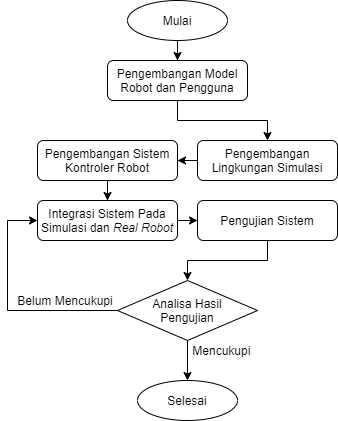
\includegraphics[scale=0.6]{gambar/blok-diagram-kerja.png}
  \caption{Blok diagram dari alur pekerjaan.}
  \label{fig:blogdiagramkerja}
\end{figure}

Kemudian, sistem robot berbasis ROS 2 akan dikembangkan.
Pengembangan sistem tersebut dilakukan secara terabstraksi yang mana nantinya akan terpisah menjadi 3 bagian,
  dimana sistem yang mengatur komponen yang ada di simulasi akan dibentuk sebagai \emph{Gazebo Plugins},
  sistem yang mengatur komponen yang ada di \emph{real robot} akan dibentuk sebagai \emph{controller node},
  dan terakhir sistem yang mengatur tindakan robot secara umum untuk simulasi dan \emph{real robot} akan dibentuk sebagai \emph{behavior node}.

Bagian akhir dari pekerjaan ini adalah pengujian untuk sistem yang telah dibuat.
Pengujian nantinya akan terdiri dari beberapa bagian yang menguji berbagai aspek yang ada pada sistem yang telah dikembangkan.
Jika hasil pengujian dirasa belum mencukupi, integrasi sistem pada simulasi dan \emph{real robot} akan dilakukan kembali hingga hasil pengujian di keduanya cukup sesuai.
Bagian ini secara lebih lanjut akan dijelaskan pada bab \ref{chap:hasilpengujian}.

\subimport{3-desain-implementasi}{1-model-robot.tex}
\subimport{3-desain-implementasi}{2-model-pengguna.tex}
\subimport{3-desain-implementasi}{3-lingkungan-simulasi.tex}
\subimport{3-desain-implementasi}{4-behavior-node.tex}
\subimport{3-desain-implementasi}{5-integrasi-plugin.tex}
\subimport{3-desain-implementasi}{6-integrasi-robot.tex}
